\chapter{Convex Lens Image Characteristics}

\section{Aim}
To find the relationship between the position of an object and the image formed by a lens

\section{Background Information}
A lens is a transparent medium that alters the direction of light passing through it. It consists of a piece of glass\slash plastic of thickness varying from the middle to the edges with spherical surfaces on one or both sides depending on the type of the lens. There are people who wear glasses which are made by lenses for different purposes such as reading, protection from sunlight and to correct eye defects. Also, there are several instruments like cameras, microscopes, and others which use lenses. Is there a relationship between the position, size and nature of the image formed and the object’s position on the principal axis? 

\section{Materials}
Convex lens, lens holder, 2 optical pins, optical bench, screen, ruler\slash meter ruler and ray box

\section{Procedure}
\begin{enumerate}
\item Set a cross using optical pins by fixing it at a hole of a ray box (see figure).
\item Fix a lens onto a lens holder.
\item Find the focal length of the lens ($f$) by focusing the light of the sun.
\item Place the lens between a screen and a ray box on an optical bench.
\item Switch on the source of light in the ray box.
\item Place the front of the ray box at a distance between $f$ and 2$f$ from the lens. Adjust the screen until a sharp image is formed on the screen. 
\item Measure the distance between the screen and lens; observe the size (magnified or diminished), orientation (upright or inverted) and nature (virtual or real) of the image on the screen. Record the data and observations.
\item Repeat procedure 6 and 7 for positions of the ray box at $f$, 2$f$ and between $f$ and the lens.
\item Tabulate your results including the position of the ray box, image distance, size, nature and the position relative to the lens of the image.
\end{enumerate}

\begin{figure}[h!]
\centering
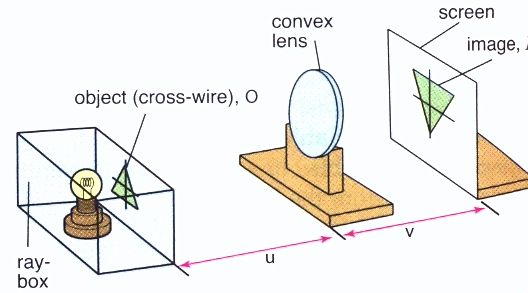
\includegraphics[width=10cm]{./img/convex-lens-1.png}
\caption{Convex Lens Image Characteristics practical setup}
\label{fig:convex-lens-1}
\end{figure}

\section{Safety Measures}
Hold the lens carefully because it breaks easily.

\section{Analysis and Interpretation}
\begin{enumerate}
\item As the object moved away from the focal distance of the lens; explain what happened to the following:
\begin{itemize}
\item[(i)] The image size;
\item[(ii)] The image orientation;
\item[(iii)] The nature of the image; and
\item[(iv)] The position of the image.
\end{itemize}

\item Calculate the theoretical values of the image distance using the lens maker’s equation for each ray box position.
\end{enumerate}

\section{Conclusion}
What are the relationships of the image size, orientation, nature, and position to an increase in object distance from the focal distance of the lens? 

\section{Questions for Discussion}
\begin{enumerate}
\item What is the size and nature of the image if the object is placed between $f$ and the lens?
\item Why might your theoretical values be different from your experimental values?
\item In absence of lenses what other materials can be used?
\end{enumerate}

\section{Reflection and Self Assessment}
\begin{enumerate}
\item What type of lens would you advise a person with long-sightedness to use?
\item What are your impressions of this experiment?
\end{enumerate}